
% Default to the notebook output style

    


% Inherit from the specified cell style.




    
\documentclass[11pt]{article}

    
    
    \usepackage[T1]{fontenc}
    % Nicer default font (+ math font) than Computer Modern for most use cases
    \usepackage{mathpazo}

    % Basic figure setup, for now with no caption control since it's done
    % automatically by Pandoc (which extracts ![](path) syntax from Markdown).
    \usepackage{graphicx}
    % We will generate all images so they have a width \maxwidth. This means
    % that they will get their normal width if they fit onto the page, but
    % are scaled down if they would overflow the margins.
    \makeatletter
    \def\maxwidth{\ifdim\Gin@nat@width>\linewidth\linewidth
    \else\Gin@nat@width\fi}
    \makeatother
    \let\Oldincludegraphics\includegraphics
    % Set max figure width to be 80% of text width, for now hardcoded.
    \renewcommand{\includegraphics}[1]{\Oldincludegraphics[width=.8\maxwidth]{#1}}
    % Ensure that by default, figures have no caption (until we provide a
    % proper Figure object with a Caption API and a way to capture that
    % in the conversion process - todo).
    \usepackage{caption}
    \DeclareCaptionLabelFormat{nolabel}{}
    \captionsetup{labelformat=nolabel}

    \usepackage{adjustbox} % Used to constrain images to a maximum size 
    \usepackage{xcolor} % Allow colors to be defined
    \usepackage{enumerate} % Needed for markdown enumerations to work
    \usepackage{geometry} % Used to adjust the document margins
    \usepackage{amsmath} % Equations
    \usepackage{amssymb} % Equations
    \usepackage{textcomp} % defines textquotesingle
    % Hack from http://tex.stackexchange.com/a/47451/13684:
    \AtBeginDocument{%
        \def\PYZsq{\textquotesingle}% Upright quotes in Pygmentized code
    }
    \usepackage{upquote} % Upright quotes for verbatim code
    \usepackage{eurosym} % defines \euro
    \usepackage[mathletters]{ucs} % Extended unicode (utf-8) support
    \usepackage[utf8x]{inputenc} % Allow utf-8 characters in the tex document
    \usepackage{fancyvrb} % verbatim replacement that allows latex
    \usepackage{grffile} % extends the file name processing of package graphics 
                         % to support a larger range 
    % The hyperref package gives us a pdf with properly built
    % internal navigation ('pdf bookmarks' for the table of contents,
    % internal cross-reference links, web links for URLs, etc.)
    \usepackage{hyperref}
    \usepackage{longtable} % longtable support required by pandoc >1.10
    \usepackage{booktabs}  % table support for pandoc > 1.12.2
    \usepackage[inline]{enumitem} % IRkernel/repr support (it uses the enumerate* environment)
    \usepackage[normalem]{ulem} % ulem is needed to support strikethroughs (\sout)
                                % normalem makes italics be italics, not underlines
    

    
    
    % Colors for the hyperref package
    \definecolor{urlcolor}{rgb}{0,.145,.698}
    \definecolor{linkcolor}{rgb}{.71,0.21,0.01}
    \definecolor{citecolor}{rgb}{.12,.54,.11}

    % ANSI colors
    \definecolor{ansi-black}{HTML}{3E424D}
    \definecolor{ansi-black-intense}{HTML}{282C36}
    \definecolor{ansi-red}{HTML}{E75C58}
    \definecolor{ansi-red-intense}{HTML}{B22B31}
    \definecolor{ansi-green}{HTML}{00A250}
    \definecolor{ansi-green-intense}{HTML}{007427}
    \definecolor{ansi-yellow}{HTML}{DDB62B}
    \definecolor{ansi-yellow-intense}{HTML}{B27D12}
    \definecolor{ansi-blue}{HTML}{208FFB}
    \definecolor{ansi-blue-intense}{HTML}{0065CA}
    \definecolor{ansi-magenta}{HTML}{D160C4}
    \definecolor{ansi-magenta-intense}{HTML}{A03196}
    \definecolor{ansi-cyan}{HTML}{60C6C8}
    \definecolor{ansi-cyan-intense}{HTML}{258F8F}
    \definecolor{ansi-white}{HTML}{C5C1B4}
    \definecolor{ansi-white-intense}{HTML}{A1A6B2}

    % commands and environments needed by pandoc snippets
    % extracted from the output of `pandoc -s`
    \providecommand{\tightlist}{%
      \setlength{\itemsep}{0pt}\setlength{\parskip}{0pt}}
    \DefineVerbatimEnvironment{Highlighting}{Verbatim}{commandchars=\\\{\}}
    % Add ',fontsize=\small' for more characters per line
    \newenvironment{Shaded}{}{}
    \newcommand{\KeywordTok}[1]{\textcolor[rgb]{0.00,0.44,0.13}{\textbf{{#1}}}}
    \newcommand{\DataTypeTok}[1]{\textcolor[rgb]{0.56,0.13,0.00}{{#1}}}
    \newcommand{\DecValTok}[1]{\textcolor[rgb]{0.25,0.63,0.44}{{#1}}}
    \newcommand{\BaseNTok}[1]{\textcolor[rgb]{0.25,0.63,0.44}{{#1}}}
    \newcommand{\FloatTok}[1]{\textcolor[rgb]{0.25,0.63,0.44}{{#1}}}
    \newcommand{\CharTok}[1]{\textcolor[rgb]{0.25,0.44,0.63}{{#1}}}
    \newcommand{\StringTok}[1]{\textcolor[rgb]{0.25,0.44,0.63}{{#1}}}
    \newcommand{\CommentTok}[1]{\textcolor[rgb]{0.38,0.63,0.69}{\textit{{#1}}}}
    \newcommand{\OtherTok}[1]{\textcolor[rgb]{0.00,0.44,0.13}{{#1}}}
    \newcommand{\AlertTok}[1]{\textcolor[rgb]{1.00,0.00,0.00}{\textbf{{#1}}}}
    \newcommand{\FunctionTok}[1]{\textcolor[rgb]{0.02,0.16,0.49}{{#1}}}
    \newcommand{\RegionMarkerTok}[1]{{#1}}
    \newcommand{\ErrorTok}[1]{\textcolor[rgb]{1.00,0.00,0.00}{\textbf{{#1}}}}
    \newcommand{\NormalTok}[1]{{#1}}
    
    % Additional commands for more recent versions of Pandoc
    \newcommand{\ConstantTok}[1]{\textcolor[rgb]{0.53,0.00,0.00}{{#1}}}
    \newcommand{\SpecialCharTok}[1]{\textcolor[rgb]{0.25,0.44,0.63}{{#1}}}
    \newcommand{\VerbatimStringTok}[1]{\textcolor[rgb]{0.25,0.44,0.63}{{#1}}}
    \newcommand{\SpecialStringTok}[1]{\textcolor[rgb]{0.73,0.40,0.53}{{#1}}}
    \newcommand{\ImportTok}[1]{{#1}}
    \newcommand{\DocumentationTok}[1]{\textcolor[rgb]{0.73,0.13,0.13}{\textit{{#1}}}}
    \newcommand{\AnnotationTok}[1]{\textcolor[rgb]{0.38,0.63,0.69}{\textbf{\textit{{#1}}}}}
    \newcommand{\CommentVarTok}[1]{\textcolor[rgb]{0.38,0.63,0.69}{\textbf{\textit{{#1}}}}}
    \newcommand{\VariableTok}[1]{\textcolor[rgb]{0.10,0.09,0.49}{{#1}}}
    \newcommand{\ControlFlowTok}[1]{\textcolor[rgb]{0.00,0.44,0.13}{\textbf{{#1}}}}
    \newcommand{\OperatorTok}[1]{\textcolor[rgb]{0.40,0.40,0.40}{{#1}}}
    \newcommand{\BuiltInTok}[1]{{#1}}
    \newcommand{\ExtensionTok}[1]{{#1}}
    \newcommand{\PreprocessorTok}[1]{\textcolor[rgb]{0.74,0.48,0.00}{{#1}}}
    \newcommand{\AttributeTok}[1]{\textcolor[rgb]{0.49,0.56,0.16}{{#1}}}
    \newcommand{\InformationTok}[1]{\textcolor[rgb]{0.38,0.63,0.69}{\textbf{\textit{{#1}}}}}
    \newcommand{\WarningTok}[1]{\textcolor[rgb]{0.38,0.63,0.69}{\textbf{\textit{{#1}}}}}
    
    
    % Define a nice break command that doesn't care if a line doesn't already
    % exist.
    \def\br{\hspace*{\fill} \\* }
    % Math Jax compatability definitions
    \def\gt{>}
    \def\lt{<}
    % Document parameters
    \title{Notebook 1}
    
    
    

    % Pygments definitions
    
\makeatletter
\def\PY@reset{\let\PY@it=\relax \let\PY@bf=\relax%
    \let\PY@ul=\relax \let\PY@tc=\relax%
    \let\PY@bc=\relax \let\PY@ff=\relax}
\def\PY@tok#1{\csname PY@tok@#1\endcsname}
\def\PY@toks#1+{\ifx\relax#1\empty\else%
    \PY@tok{#1}\expandafter\PY@toks\fi}
\def\PY@do#1{\PY@bc{\PY@tc{\PY@ul{%
    \PY@it{\PY@bf{\PY@ff{#1}}}}}}}
\def\PY#1#2{\PY@reset\PY@toks#1+\relax+\PY@do{#2}}

\expandafter\def\csname PY@tok@w\endcsname{\def\PY@tc##1{\textcolor[rgb]{0.73,0.73,0.73}{##1}}}
\expandafter\def\csname PY@tok@c\endcsname{\let\PY@it=\textit\def\PY@tc##1{\textcolor[rgb]{0.25,0.50,0.50}{##1}}}
\expandafter\def\csname PY@tok@cp\endcsname{\def\PY@tc##1{\textcolor[rgb]{0.74,0.48,0.00}{##1}}}
\expandafter\def\csname PY@tok@k\endcsname{\let\PY@bf=\textbf\def\PY@tc##1{\textcolor[rgb]{0.00,0.50,0.00}{##1}}}
\expandafter\def\csname PY@tok@kp\endcsname{\def\PY@tc##1{\textcolor[rgb]{0.00,0.50,0.00}{##1}}}
\expandafter\def\csname PY@tok@kt\endcsname{\def\PY@tc##1{\textcolor[rgb]{0.69,0.00,0.25}{##1}}}
\expandafter\def\csname PY@tok@o\endcsname{\def\PY@tc##1{\textcolor[rgb]{0.40,0.40,0.40}{##1}}}
\expandafter\def\csname PY@tok@ow\endcsname{\let\PY@bf=\textbf\def\PY@tc##1{\textcolor[rgb]{0.67,0.13,1.00}{##1}}}
\expandafter\def\csname PY@tok@nb\endcsname{\def\PY@tc##1{\textcolor[rgb]{0.00,0.50,0.00}{##1}}}
\expandafter\def\csname PY@tok@nf\endcsname{\def\PY@tc##1{\textcolor[rgb]{0.00,0.00,1.00}{##1}}}
\expandafter\def\csname PY@tok@nc\endcsname{\let\PY@bf=\textbf\def\PY@tc##1{\textcolor[rgb]{0.00,0.00,1.00}{##1}}}
\expandafter\def\csname PY@tok@nn\endcsname{\let\PY@bf=\textbf\def\PY@tc##1{\textcolor[rgb]{0.00,0.00,1.00}{##1}}}
\expandafter\def\csname PY@tok@ne\endcsname{\let\PY@bf=\textbf\def\PY@tc##1{\textcolor[rgb]{0.82,0.25,0.23}{##1}}}
\expandafter\def\csname PY@tok@nv\endcsname{\def\PY@tc##1{\textcolor[rgb]{0.10,0.09,0.49}{##1}}}
\expandafter\def\csname PY@tok@no\endcsname{\def\PY@tc##1{\textcolor[rgb]{0.53,0.00,0.00}{##1}}}
\expandafter\def\csname PY@tok@nl\endcsname{\def\PY@tc##1{\textcolor[rgb]{0.63,0.63,0.00}{##1}}}
\expandafter\def\csname PY@tok@ni\endcsname{\let\PY@bf=\textbf\def\PY@tc##1{\textcolor[rgb]{0.60,0.60,0.60}{##1}}}
\expandafter\def\csname PY@tok@na\endcsname{\def\PY@tc##1{\textcolor[rgb]{0.49,0.56,0.16}{##1}}}
\expandafter\def\csname PY@tok@nt\endcsname{\let\PY@bf=\textbf\def\PY@tc##1{\textcolor[rgb]{0.00,0.50,0.00}{##1}}}
\expandafter\def\csname PY@tok@nd\endcsname{\def\PY@tc##1{\textcolor[rgb]{0.67,0.13,1.00}{##1}}}
\expandafter\def\csname PY@tok@s\endcsname{\def\PY@tc##1{\textcolor[rgb]{0.73,0.13,0.13}{##1}}}
\expandafter\def\csname PY@tok@sd\endcsname{\let\PY@it=\textit\def\PY@tc##1{\textcolor[rgb]{0.73,0.13,0.13}{##1}}}
\expandafter\def\csname PY@tok@si\endcsname{\let\PY@bf=\textbf\def\PY@tc##1{\textcolor[rgb]{0.73,0.40,0.53}{##1}}}
\expandafter\def\csname PY@tok@se\endcsname{\let\PY@bf=\textbf\def\PY@tc##1{\textcolor[rgb]{0.73,0.40,0.13}{##1}}}
\expandafter\def\csname PY@tok@sr\endcsname{\def\PY@tc##1{\textcolor[rgb]{0.73,0.40,0.53}{##1}}}
\expandafter\def\csname PY@tok@ss\endcsname{\def\PY@tc##1{\textcolor[rgb]{0.10,0.09,0.49}{##1}}}
\expandafter\def\csname PY@tok@sx\endcsname{\def\PY@tc##1{\textcolor[rgb]{0.00,0.50,0.00}{##1}}}
\expandafter\def\csname PY@tok@m\endcsname{\def\PY@tc##1{\textcolor[rgb]{0.40,0.40,0.40}{##1}}}
\expandafter\def\csname PY@tok@gh\endcsname{\let\PY@bf=\textbf\def\PY@tc##1{\textcolor[rgb]{0.00,0.00,0.50}{##1}}}
\expandafter\def\csname PY@tok@gu\endcsname{\let\PY@bf=\textbf\def\PY@tc##1{\textcolor[rgb]{0.50,0.00,0.50}{##1}}}
\expandafter\def\csname PY@tok@gd\endcsname{\def\PY@tc##1{\textcolor[rgb]{0.63,0.00,0.00}{##1}}}
\expandafter\def\csname PY@tok@gi\endcsname{\def\PY@tc##1{\textcolor[rgb]{0.00,0.63,0.00}{##1}}}
\expandafter\def\csname PY@tok@gr\endcsname{\def\PY@tc##1{\textcolor[rgb]{1.00,0.00,0.00}{##1}}}
\expandafter\def\csname PY@tok@ge\endcsname{\let\PY@it=\textit}
\expandafter\def\csname PY@tok@gs\endcsname{\let\PY@bf=\textbf}
\expandafter\def\csname PY@tok@gp\endcsname{\let\PY@bf=\textbf\def\PY@tc##1{\textcolor[rgb]{0.00,0.00,0.50}{##1}}}
\expandafter\def\csname PY@tok@go\endcsname{\def\PY@tc##1{\textcolor[rgb]{0.53,0.53,0.53}{##1}}}
\expandafter\def\csname PY@tok@gt\endcsname{\def\PY@tc##1{\textcolor[rgb]{0.00,0.27,0.87}{##1}}}
\expandafter\def\csname PY@tok@err\endcsname{\def\PY@bc##1{\setlength{\fboxsep}{0pt}\fcolorbox[rgb]{1.00,0.00,0.00}{1,1,1}{\strut ##1}}}
\expandafter\def\csname PY@tok@kc\endcsname{\let\PY@bf=\textbf\def\PY@tc##1{\textcolor[rgb]{0.00,0.50,0.00}{##1}}}
\expandafter\def\csname PY@tok@kd\endcsname{\let\PY@bf=\textbf\def\PY@tc##1{\textcolor[rgb]{0.00,0.50,0.00}{##1}}}
\expandafter\def\csname PY@tok@kn\endcsname{\let\PY@bf=\textbf\def\PY@tc##1{\textcolor[rgb]{0.00,0.50,0.00}{##1}}}
\expandafter\def\csname PY@tok@kr\endcsname{\let\PY@bf=\textbf\def\PY@tc##1{\textcolor[rgb]{0.00,0.50,0.00}{##1}}}
\expandafter\def\csname PY@tok@bp\endcsname{\def\PY@tc##1{\textcolor[rgb]{0.00,0.50,0.00}{##1}}}
\expandafter\def\csname PY@tok@fm\endcsname{\def\PY@tc##1{\textcolor[rgb]{0.00,0.00,1.00}{##1}}}
\expandafter\def\csname PY@tok@vc\endcsname{\def\PY@tc##1{\textcolor[rgb]{0.10,0.09,0.49}{##1}}}
\expandafter\def\csname PY@tok@vg\endcsname{\def\PY@tc##1{\textcolor[rgb]{0.10,0.09,0.49}{##1}}}
\expandafter\def\csname PY@tok@vi\endcsname{\def\PY@tc##1{\textcolor[rgb]{0.10,0.09,0.49}{##1}}}
\expandafter\def\csname PY@tok@vm\endcsname{\def\PY@tc##1{\textcolor[rgb]{0.10,0.09,0.49}{##1}}}
\expandafter\def\csname PY@tok@sa\endcsname{\def\PY@tc##1{\textcolor[rgb]{0.73,0.13,0.13}{##1}}}
\expandafter\def\csname PY@tok@sb\endcsname{\def\PY@tc##1{\textcolor[rgb]{0.73,0.13,0.13}{##1}}}
\expandafter\def\csname PY@tok@sc\endcsname{\def\PY@tc##1{\textcolor[rgb]{0.73,0.13,0.13}{##1}}}
\expandafter\def\csname PY@tok@dl\endcsname{\def\PY@tc##1{\textcolor[rgb]{0.73,0.13,0.13}{##1}}}
\expandafter\def\csname PY@tok@s2\endcsname{\def\PY@tc##1{\textcolor[rgb]{0.73,0.13,0.13}{##1}}}
\expandafter\def\csname PY@tok@sh\endcsname{\def\PY@tc##1{\textcolor[rgb]{0.73,0.13,0.13}{##1}}}
\expandafter\def\csname PY@tok@s1\endcsname{\def\PY@tc##1{\textcolor[rgb]{0.73,0.13,0.13}{##1}}}
\expandafter\def\csname PY@tok@mb\endcsname{\def\PY@tc##1{\textcolor[rgb]{0.40,0.40,0.40}{##1}}}
\expandafter\def\csname PY@tok@mf\endcsname{\def\PY@tc##1{\textcolor[rgb]{0.40,0.40,0.40}{##1}}}
\expandafter\def\csname PY@tok@mh\endcsname{\def\PY@tc##1{\textcolor[rgb]{0.40,0.40,0.40}{##1}}}
\expandafter\def\csname PY@tok@mi\endcsname{\def\PY@tc##1{\textcolor[rgb]{0.40,0.40,0.40}{##1}}}
\expandafter\def\csname PY@tok@il\endcsname{\def\PY@tc##1{\textcolor[rgb]{0.40,0.40,0.40}{##1}}}
\expandafter\def\csname PY@tok@mo\endcsname{\def\PY@tc##1{\textcolor[rgb]{0.40,0.40,0.40}{##1}}}
\expandafter\def\csname PY@tok@ch\endcsname{\let\PY@it=\textit\def\PY@tc##1{\textcolor[rgb]{0.25,0.50,0.50}{##1}}}
\expandafter\def\csname PY@tok@cm\endcsname{\let\PY@it=\textit\def\PY@tc##1{\textcolor[rgb]{0.25,0.50,0.50}{##1}}}
\expandafter\def\csname PY@tok@cpf\endcsname{\let\PY@it=\textit\def\PY@tc##1{\textcolor[rgb]{0.25,0.50,0.50}{##1}}}
\expandafter\def\csname PY@tok@c1\endcsname{\let\PY@it=\textit\def\PY@tc##1{\textcolor[rgb]{0.25,0.50,0.50}{##1}}}
\expandafter\def\csname PY@tok@cs\endcsname{\let\PY@it=\textit\def\PY@tc##1{\textcolor[rgb]{0.25,0.50,0.50}{##1}}}

\def\PYZbs{\char`\\}
\def\PYZus{\char`\_}
\def\PYZob{\char`\{}
\def\PYZcb{\char`\}}
\def\PYZca{\char`\^}
\def\PYZam{\char`\&}
\def\PYZlt{\char`\<}
\def\PYZgt{\char`\>}
\def\PYZsh{\char`\#}
\def\PYZpc{\char`\%}
\def\PYZdl{\char`\$}
\def\PYZhy{\char`\-}
\def\PYZsq{\char`\'}
\def\PYZdq{\char`\"}
\def\PYZti{\char`\~}
% for compatibility with earlier versions
\def\PYZat{@}
\def\PYZlb{[}
\def\PYZrb{]}
\makeatother


    % Exact colors from NB
    \definecolor{incolor}{rgb}{0.0, 0.0, 0.5}
    \definecolor{outcolor}{rgb}{0.545, 0.0, 0.0}



    
    % Prevent overflowing lines due to hard-to-break entities
    \sloppy 
    % Setup hyperref package
    \hypersetup{
      breaklinks=true,  % so long urls are correctly broken across lines
      colorlinks=true,
      urlcolor=urlcolor,
      linkcolor=linkcolor,
      citecolor=citecolor,
      }
    % Slightly bigger margins than the latex defaults
    
    \geometry{verbose,tmargin=1in,bmargin=1in,lmargin=1in,rmargin=1in}
    
    

    \begin{document}
    
    
    \maketitle
    
    

    
    Table of Contents{}

{{1~~}Data Science for ALMA}

{{1.1~~}Notebook 1: inspecting the Archive and introduction to pandas}

{{1.2~~}Useful resources}

{{1.2.1~~}Jupyter notebooks}

{{1.2.2~~}Conda environments}

{{1.2.3~~}cx\_Oracle library}

{{1.2.4~~}Pandas}

{{1.2.5~~}Online classes}

{{1.2.6~~}Cheat Sheets}

{{1.3~~}Creating and managing the conda environment for your training}

{{1.4~~}Using cx\_Oracle and pandas to inspect the Archive}

{{1.4.1~~}Querying for all the available Tables}

{{1.4.2~~}First pandas's inspection methods}

{{1.4.2.1~~}.info()}

{{1.4.2.2~~}.head() and .tail()}

{{1.4.2.3~~}.describe()}

{{1.4.2.4~~}Accessing/selecting columns and rows}

{{1.4.2.5~~}Pandas columns/rows as Series}

{{1.4.3~~}Going Back to the all\_tables\_df}

    \section{Data Science for ALMA}\label{data-science-for-alma}

\subsection{Notebook 1: inspecting the Archive and introduction to
pandas}\label{notebook-1-inspecting-the-archive-and-introduction-to-pandas}

This is the first notebook in a series to train ourselves in data
science projects. The goals are:

\begin{enumerate}
\def\labelenumi{\arabic{enumi}.}
\tightlist
\item
  Familiarize with Jupyter notebooks
\item
  Create your first local conda environment
\item
  Connect to the Archive using \texttt{cx\_Oracle}
\item
  Introduction to pandas methods
\end{enumerate}

\subsection{Useful resources}\label{useful-resources}

\subsubsection{Jupyter notebooks}\label{jupyter-notebooks}

\begin{itemize}
\tightlist
\item
  The official documentation can be found at this
  \href{http://jupyter-notebook.readthedocs.io/en/stable/}{Jupyter
  Notebooks}
\item
  Some simple tutorials:
\item
  \href{https://www.dataquest.io/blog/jupyter-notebook-tutorial/}{Jupyter
  Notebook for Beginners: A Tutorial}
\item
  \href{https://codingthesmartway.com/getting-started-with-jupyter-notebook-for-python/}{Getting
  Started with jupyter notebook for python}
\item
  \href{https://plot.ly/python/ipython-notebook-tutorial/}{Plotly with
  Jupyter Notebooks}, a more ad-hoc tutorial aimed to the use of the
  plotly library for visualizations, but is a nice example of advanced
  uses.
\item
  \href{https://www.dataquest.io/blog/jupyter-notebook-tips-tricks-shortcuts/}{Jupyter
  Notebook tips, tricks, and shortcuts}, a great resource for tips and
  hints!
\item
  Extending Jupyter Notebooks
\end{itemize}

\subsubsection{Conda environments}\label{conda-environments}

We will use the Jupyter Hub interface to create a conda environment for
this notebook, but the original documentation to manage \emph{conda} can
be found
\href{https://conda.io/docs/user-guide/tasks/manage-environments.html}{here}.
From there you can also access the full documentation for
(ana)\href{https://conda.io/docs/index.html}{conda}

\subsubsection{\texorpdfstring{\texttt{cx\_Oracle}
library}{cx\_Oracle library}}\label{cx_oracle-library}

The documentation and resources are much more sparse. Usually, google
search and links to
\href{https://stackoverflow.com/search?q=cx_Oracle}{stackoverflow} will
be your best guide.

Yet, the official documentation is at this
\href{http://cx-oracle.readthedocs.io/en/latest/}{link}, and
\href{https://github.com/oracle/python-cx_Oracle/tree/master/samples}{some
advanced samples here}.

\subsubsection{Pandas}\label{pandas}

The amount of tutorials and introductions to pandas is just
overwhelming. Here is just a personal selection:

\begin{itemize}
\tightlist
\item
  Official documentation for the latest version
  \href{http://pandas.pydata.org/pandas-docs/stable/}{here}
\item
  Official quick guide:
  \href{http://pandas.pydata.org/pandas-docs/stable/10min.html}{10
  Minutes to pandas}
\item
  Cookbook: \href{https://github.com/jvns/pandas-cookbook}{Pandas
  cookbook}
\item
  \href{http://wavedatalab.github.io/datawithpython/index.html}{Python
  for data science}
\item
  Official list of tutorials:
  \href{http://pandas.pydata.org/pandas-docs/stable/tutorials.html}{Tutorials}
\end{itemize}

\subsubsection{Online classes}\label{online-classes}

If you think you can get some support from ALMA to pay for some online
traing, then check out:

\begin{itemize}
\tightlist
\item
  Datacamp:
  \href{https://www.datacamp.com/tracks/data-scientist-with-python}{Data
  Scientist with Python} track.
\item
  edX: \href{https://www.edx.org/micromasters/data-science}{Data Science
  micromaster} (All four classes can be audited for free! Meaning you
  can get all the class materials, but you don't get any certificates)
\item
  Coursera:
  \href{https://courses.edx.org/course_modes/choose/course-v1:UCSanDiegoX+DSE210x+1T2018/}{Applied
  Data Science with Python Specialization}. A trial is available.
\end{itemize}

\subsubsection{Cheat Sheets}\label{cheat-sheets}

\begin{itemize}
\tightlist
\item
  \href{http://datacamp-community.s3.amazonaws.com/50d31142-3de0-4159-89b9-18b718a728ef}{Importing
  Data with Python}
\item
  \href{http://datacamp-community.s3.amazonaws.com/fbc502d0-46b2-4e1b-b6b0-5402ff273251}{Pandas
  Cheat sheet}
\item
  \href{http://datacamp-community.s3.amazonaws.com/48093c40-5303-45f4-bbf9-0c96c0133c40}{Jupyter
  Notebook Cheat Sheet}
\item
  \href{http://datacamp-community.s3.amazonaws.com/9f0f2ae1-8bd8-4302-a67b-e17f3059d9e8}{Pandas
  Cheat Sheet: Data Wrangling in Python}
\end{itemize}

\subsection{Creating and managing the conda environment for your
training}\label{creating-and-managing-the-conda-environment-for-your-training}

While we've seen that there is an interface to manage your conda
environments within your jupyter server, we will use the terminal
interface to create an environment to use in our training notebooks, the
reason being that the integrated interface is kind of buggy still
(useful to add packages or libraries, but not working good enough to
create or clone environments)

1.- Go to your \texttt{Home} jupyter browser tab:

    

    2.- Open a terminal. The new terminal will open in new browser tab:

    

    Like this

    

    3.- In the terminal run
\texttt{cp\ /etc/jupyterhub/Notebooks/datascience3.txt\ .} to copy a
file that has the definitions to create a conda environment with the
same specs as the one used to originally create this notebook (feel free
to check its contents, and check the
\href{https://conda.io/docs/index.html}{conda documentation} to learn
more).

4.- Create the new conda enviroment in the terminal:
\texttt{conda\ env\ create\ -n\ datascience3\ -f\ datascience3.txt}.
What this command does is to create a new conda environment called
\texttt{datascience3} (option -n) using the specifications detailed in
the file \texttt{datascience3} (option -f). Wait for the command to end.

5.- It is a good practice, to save space, to run
\texttt{conda\ clean\ -\/-all} after you create an environment or after
you add or update new packages or libraries. This will clean the cache
of all the downloaded files.

6.- If you were to work with python in the command line, to activate the
new environment you would run \texttt{source\ activate\ datascience3}.
To deactivate the environment and go back to the root environment, you
just need to run \texttt{source\ deactivate}

7.- Shutdown the terminal by execution \texttt{exit} and closing the
terminal tab in your browser.

For our first exercise we are almost done. The only reminding step is to
set the kernel for this notebook to be the one provided by your knew
\texttt{datascience3} environment, using the menu at the top of the
notebook
\texttt{Kernel\ \textgreater{}\ Change\ Kernel\ \textgreater{}\ Python\ {[}conda\ env:datascience3{]}}.
Now, in your home tab, you should also be capable of creating new
notebooks with the new Kernel.

\textbf{If you don't see the new Kernel as an option}: Save and close
this notebook (\texttt{File\ \textgreater{}\ Save\ and\ Checkpoint} and
then \texttt{File\ \textgreater{}\ Close\ and\ Halt}). Now logout form
the Jupyter server by pressing \texttt{Logout} in the top right corner,
log in again, and open this notebook to continue.

\subsection{Using cx\_Oracle and pandas to inspect the
Archive}\label{using-cx_oracle-and-pandas-to-inspect-the-archive}

\subsubsection{Querying for all the available
Tables}\label{querying-for-all-the-available-tables}

We will start by loading the libraries, read a \emph{connection string}
(to be discussed live in our next session), and open a connection to the
read-only version of the archive.

    \begin{Verbatim}[commandchars=\\\{\}]
{\color{incolor}In [{\color{incolor}1}]:} \PY{c+c1}{\PYZsh{} Any line beggining in a code\PYZhy{}cel with a \PYZsh{} is a comment line, and won\PYZsq{}t be }
        \PY{c+c1}{\PYZsh{} executed}
        
        \PY{k+kn}{import} \PY{n+nn}{os}
        \PY{k+kn}{import} \PY{n+nn}{pandas} \PY{k}{as} \PY{n+nn}{pd}
        \PY{k+kn}{import} \PY{n+nn}{cx\PYZus{}Oracle}
        
        \PY{n}{connection\PYZus{}string} \PY{o}{=} \PY{n}{os}\PY{o}{.}\PY{n}{environ}\PY{p}{[}\PY{l+s+s1}{\PYZsq{}}\PY{l+s+s1}{CON\PYZus{}STR}\PY{l+s+s1}{\PYZsq{}}\PY{p}{]}
\end{Verbatim}


    \begin{Verbatim}[commandchars=\\\{\}]
{\color{incolor}In [{\color{incolor}2}]:} \PY{c+c1}{\PYZsh{} Create connection to the read\PYZhy{}only DB}
        \PY{n}{con} \PY{o}{=} \PY{n}{cx\PYZus{}Oracle}\PY{o}{.}\PY{n}{connect}\PY{p}{(}\PY{n}{connection\PYZus{}string}\PY{p}{)}
\end{Verbatim}


    \begin{Verbatim}[commandchars=\\\{\}]
{\color{incolor}In [{\color{incolor}3}]:} \PY{c+c1}{\PYZsh{} Create a cursor to do SQL queries. The cursor is the object that is used to do }
        \PY{c+c1}{\PYZsh{} queries to the archive}
        \PY{n}{cur} \PY{o}{=} \PY{n}{con}\PY{o}{.}\PY{n}{cursor}\PY{p}{(}\PY{p}{)}
\end{Verbatim}


    To execute an SQL query we use the \texttt{execute} method of the
\texttt{cur} object we just created (\texttt{cur.execute()}). The SQL
queries are strings. For example, let's query for all the available
tables in the archive. The query string we will store in
\texttt{sql\_all\_tables}

    \begin{Verbatim}[commandchars=\\\{\}]
{\color{incolor}In [{\color{incolor}4}]:} \PY{n}{sql\PYZus{}all\PYZus{}tables} \PY{o}{=} \PY{l+s+s2}{\PYZdq{}\PYZdq{}\PYZdq{}}
        \PY{l+s+s2}{SELECT DISTINCT OWNER, OBJECT\PYZus{}NAME, OBJECT\PYZus{}TYPE}
        \PY{l+s+s2}{  FROM ALL\PYZus{}OBJECTS}
        \PY{l+s+s2}{ WHERE OBJECT\PYZus{}TYPE = }\PY{l+s+s2}{\PYZsq{}}\PY{l+s+s2}{TABLE}\PY{l+s+s2}{\PYZsq{}}
        \PY{l+s+s2}{\PYZdq{}\PYZdq{}\PYZdq{}}
\end{Verbatim}


    Next, we request to the database to execute the query:

    \begin{Verbatim}[commandchars=\\\{\}]
{\color{incolor}In [{\color{incolor} }]:} \PY{n}{cur}\PY{o}{.}\PY{n}{execute}\PY{p}{(}\PY{n}{sql\PYZus{}all\PYZus{}tables}\PY{p}{)}
\end{Verbatim}


    And to get the results we use the method \texttt{fetchall}:

    \begin{Verbatim}[commandchars=\\\{\}]
{\color{incolor}In [{\color{incolor} }]:} \PY{n}{cur}\PY{o}{.}\PY{n}{fetchall}\PY{p}{(}\PY{p}{)}
\end{Verbatim}


    \texttt{fetchall} returns the query results in a list, each row
represented by a tuple, with one element by each column queried. It is
important to notice that once we have requested the results from the
query, execution \texttt{fetchall} once more will produce not results:

    \begin{Verbatim}[commandchars=\\\{\}]
{\color{incolor}In [{\color{incolor} }]:} \PY{n}{cur}\PY{o}{.}\PY{n}{fetchall}\PY{p}{(}\PY{p}{)}
\end{Verbatim}


    So, to get again the results one needs to run \texttt{cur.execute}
again, followed by the \texttt{cur.fetchall} call.

We have not stored the results in any local variable yet. Let's do that.
But since we want to start using pandas, we will store the results in a
pandas Dataframe, which is one of the two data structures provided by
\texttt{pandas}:

\begin{figure}
\centering
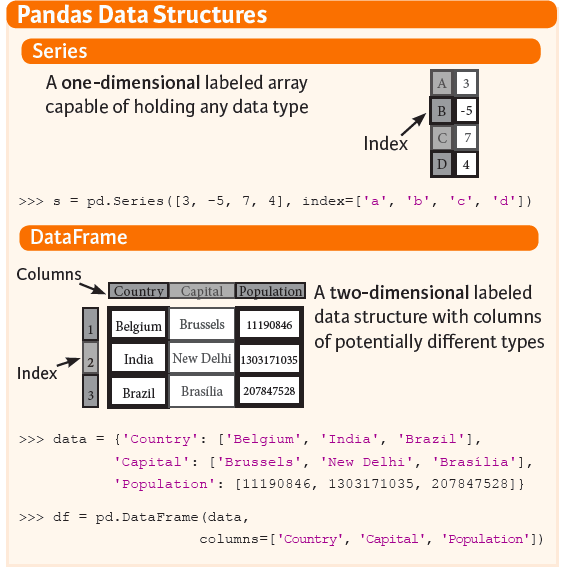
\includegraphics{img/pandas-02.png}
\caption{img}
\end{figure}

(see
\href{http://pandas.pydata.org/pandas-docs/stable/overview.html\#data-structures}{pandas
data structures} and
\href{http://pandas.pydata.org/pandas-docs/stable/index.html}{pandas
documentation} in general for a full description of a Dataframe).

How do we create a dataframe to store the queries' results?

    \begin{Verbatim}[commandchars=\\\{\}]
{\color{incolor}In [{\color{incolor}5}]:} \PY{c+c1}{\PYZsh{} execute query again}
        \PY{n}{cur}\PY{o}{.}\PY{n}{execute}\PY{p}{(}\PY{n}{sql\PYZus{}all\PYZus{}tables}\PY{p}{)}
        \PY{c+c1}{\PYZsh{} fetch the results and use them to create the dataframe}
        \PY{n}{all\PYZus{}tables\PYZus{}df} \PY{o}{=} \PY{n}{pd}\PY{o}{.}\PY{n}{DataFrame}\PY{p}{(}
            \PY{n}{cur}\PY{o}{.}\PY{n}{fetchall}\PY{p}{(}\PY{p}{)}\PY{p}{,} \PY{n}{columns}\PY{o}{=}\PY{p}{[}\PY{n}{rec}\PY{p}{[}\PY{l+m+mi}{0}\PY{p}{]} \PY{k}{for} \PY{n}{rec} \PY{o+ow}{in} \PY{n}{cur}\PY{o}{.}\PY{n}{description}\PY{p}{]}\PY{p}{)}
\end{Verbatim}


    Creating a pandas DataFrame is done by calling \texttt{pd.Dataframes}. A
dataframe can be created with multiple kinds of iterables (lists,
tuples, sets, numpy arrays, etc.): in this case we are using the list of
tuples that is returned by \texttt{cur.fetchall}. The second named
argument, \texttt{columns={[}some\_list{]}}, is used to set the names
for the columns of the Dataframe. T

In this case the names of the columns were created using the
\href{https://docs.python.org/2/tutorial/datastructures.html\#list-comprehensions}{list
comprehension} \texttt{{[}rec{[}0{]}\ for\ rec\ in\ cur.description{]}}.
It is left as an exercise workout what exactly is going on here, but
\textbf{this is a method that you can use every time you create a
dataframe from a cx\_oracle query}.

\subsubsection{\texorpdfstring{First \texttt{pandas}'s inspection
methods}{First pandas's inspection methods}}\label{first-pandass-inspection-methods}

\paragraph{\texorpdfstring{\texttt{.info()}}{.info()}}\label{info}

Returns the number of entries of a dataframe, the number of columns,
their names, how many non-null entries they have, and their variable
types. Last, the memory usage of the tables is also returned

    \begin{Verbatim}[commandchars=\\\{\}]
{\color{incolor}In [{\color{incolor}6}]:} \PY{n}{all\PYZus{}tables\PYZus{}df}\PY{o}{.}\PY{n}{info}\PY{p}{(}\PY{p}{)}
\end{Verbatim}


    \begin{Verbatim}[commandchars=\\\{\}]
<class 'pandas.core.frame.DataFrame'>
RangeIndex: 2776 entries, 0 to 2775
Data columns (total 3 columns):
OWNER          2776 non-null object
OBJECT\_NAME    2776 non-null object
OBJECT\_TYPE    2776 non-null object
dtypes: object(3)
memory usage: 65.1+ KB

    \end{Verbatim}

    \textbf{Hint} The best way to understand new methods or functions in
python, is by accessing their documentation (if they are available).
There is a very useful notebook magic that allows one to quickly access
the help. Try running the next statement in a code cell:

\begin{verbatim}
?all_tables_df.info
\end{verbatim}

(there is also a keyboard shortcut (double pressing \texttt{shift-Tab})
to do the same magic without using a \texttt{?})

\paragraph{\texorpdfstring{\texttt{.head()} and
\texttt{.tail()}}{.head() and .tail()}}\label{head-and-.tail}

Return the first rows (\texttt{head}) or the last rows (\texttt{tail})
of a dataframe. By default 5 rows are returned, but you can optionally
give the number of rows to return (e.g., \texttt{.head(10)})

    \begin{Verbatim}[commandchars=\\\{\}]
{\color{incolor}In [{\color{incolor}7}]:} \PY{n}{all\PYZus{}tables\PYZus{}df}\PY{o}{.}\PY{n}{head}\PY{p}{(}\PY{p}{)}
\end{Verbatim}


\begin{Verbatim}[commandchars=\\\{\}]
{\color{outcolor}Out[{\color{outcolor}7}]:}   OWNER OBJECT\_NAME OBJECT\_TYPE
        0   SYS       CCOL\$       TABLE
        1   SYS  BOOTSTRAP\$       TABLE
        2   SYS        UET\$       TABLE
        3   SYS    HISTGRM\$       TABLE
        4   SYS  HIST\_HEAD\$       TABLE
\end{Verbatim}
            
    \begin{Verbatim}[commandchars=\\\{\}]
{\color{incolor}In [{\color{incolor}8}]:} \PY{n}{all\PYZus{}tables\PYZus{}df}\PY{o}{.}\PY{n}{tail}\PY{p}{(}\PY{l+m+mi}{10}\PY{p}{)}
\end{Verbatim}


\begin{Verbatim}[commandchars=\\\{\}]
{\color{outcolor}Out[{\color{outcolor}8}]:}                 OWNER                   OBJECT\_NAME OBJECT\_TYPE
        2766              TMC                       LODELAY       TABLE
        2767        DASHBOARD          DASHBOARD\_CORRELATOR       TABLE
        2768  SOURCECATALOGUE           MEASUREMENT\_HISTORY       TABLE
        2769              TMC               ASSEMBLYSTARTUP       TABLE
        2770              TMC                   BASEELEMENT       TABLE
        2771              TMC               TT\_05\_AR\_PARAMS       TABLE
        2772              SYS        KUPC\$DATAPUMP\_QUETAB\_2       TABLE
        2773         OGGADMIN       AQ\$\_OGG\$Q\_TAB\_EALMABB\_L       TABLE
        2774              SYS  AQ\$\_KUPC\$DATAPUMP\_QUETAB\_2\_P       TABLE
        2775              SYS            AQ\_SRVNTFN\_TABLE\_1       TABLE
\end{Verbatim}
            
    \paragraph{\texorpdfstring{\texttt{.describe()}}{.describe()}}\label{describe}

From the \texttt{docstring}:

\begin{quote}
Generates descriptive statistics that summarize the central tendency,
dispersion and shape of a dataset's distribution, excluding \texttt{NaN}
values.

Analyzes both numeric and object series, as well as \texttt{DataFrame}
column sets of mixed data types. The output will vary depending on what
is provided.
\end{quote}

    \begin{Verbatim}[commandchars=\\\{\}]
{\color{incolor}In [{\color{incolor}9}]:} \PY{n}{all\PYZus{}tables\PYZus{}df}\PY{o}{.}\PY{n}{describe}\PY{p}{(}\PY{p}{)}
\end{Verbatim}


\begin{Verbatim}[commandchars=\\\{\}]
{\color{outcolor}Out[{\color{outcolor}9}]:}        OWNER         OBJECT\_NAME OBJECT\_TYPE
        count   2776                2776        2776
        unique    28                2744           1
        top      SYS  DBMAINTAIN\_SCRIPTS       TABLE
        freq    1538                   8        2776
\end{Verbatim}
            
    \paragraph{Accessing/selecting columns and
rows}\label{accessingselecting-columns-and-rows}

    \begin{Verbatim}[commandchars=\\\{\}]
{\color{incolor}In [{\color{incolor} }]:} \PY{c+c1}{\PYZsh{} Accessing a column:}
        \PY{n}{all\PYZus{}tables\PYZus{}df}\PY{o}{.}\PY{n}{OBJECT\PYZus{}NAME}
\end{Verbatim}


    \begin{Verbatim}[commandchars=\\\{\}]
{\color{incolor}In [{\color{incolor} }]:} \PY{c+c1}{\PYZsh{} It is the same as:}
        \PY{n}{all\PYZus{}tables\PYZus{}df}\PY{o}{.}\PY{n}{loc}\PY{p}{[}\PY{p}{:}\PY{p}{,} \PY{l+s+s1}{\PYZsq{}}\PY{l+s+s1}{OBJECT\PYZus{}NAME}\PY{l+s+s1}{\PYZsq{}}\PY{p}{]}
\end{Verbatim}


    \begin{Verbatim}[commandchars=\\\{\}]
{\color{incolor}In [{\color{incolor} }]:} \PY{c+c1}{\PYZsh{} Or it could be access by the position of the column (as usual starting from 0)}
        \PY{n}{all\PYZus{}tables\PYZus{}df}\PY{o}{.}\PY{n}{iloc}\PY{p}{[}\PY{p}{:}\PY{p}{,} \PY{l+m+mi}{1}\PY{p}{]}
\end{Verbatim}


    \begin{Verbatim}[commandchars=\\\{\}]
{\color{incolor}In [{\color{incolor} }]:} \PY{c+c1}{\PYZsh{} To access a particular row, we can use the index name:}
        \PY{n}{all\PYZus{}tables\PYZus{}df}\PY{o}{.}\PY{n}{loc}\PY{p}{[}\PY{l+m+mi}{0}\PY{p}{]}
\end{Verbatim}


    \begin{Verbatim}[commandchars=\\\{\}]
{\color{incolor}In [{\color{incolor} }]:} \PY{c+c1}{\PYZsh{} To access a particular row, we use the index position:}
        \PY{n}{all\PYZus{}tables\PYZus{}df}\PY{o}{.}\PY{n}{iloc}\PY{p}{[}\PY{l+m+mi}{0}\PY{p}{]}
\end{Verbatim}


    \begin{Verbatim}[commandchars=\\\{\}]
{\color{incolor}In [{\color{incolor} }]:} \PY{c+c1}{\PYZsh{} In this previous case the positional index is the same as the name of the index}
        \PY{c+c1}{\PYZsh{} To see the difference, let\PYZsq{}s create a new dataframe with just the last 5 rows:}
        \PY{n}{df} \PY{o}{=} \PY{n}{all\PYZus{}tables\PYZus{}df}\PY{o}{.}\PY{n}{tail}\PY{p}{(}\PY{p}{)}
\end{Verbatim}


    \begin{Verbatim}[commandchars=\\\{\}]
{\color{incolor}In [{\color{incolor} }]:} \PY{c+c1}{\PYZsh{} Access the first row by positional index:}
        \PY{n}{df}\PY{o}{.}\PY{n}{iloc}\PY{p}{[}\PY{l+m+mi}{0}\PY{p}{]}
\end{Verbatim}


    \begin{Verbatim}[commandchars=\\\{\}]
{\color{incolor}In [{\color{incolor} }]:} \PY{c+c1}{\PYZsh{} The index name of the previous row can be recovered with:}
        \PY{n}{index\PYZus{}name} \PY{o}{=} \PY{n}{df}\PY{o}{.}\PY{n}{iloc}\PY{p}{[}\PY{l+m+mi}{0}\PY{p}{]}\PY{o}{.}\PY{n}{name}
        \PY{n+nb}{print}\PY{p}{(}\PY{n}{index\PYZus{}name}\PY{p}{)}
\end{Verbatim}


    \begin{Verbatim}[commandchars=\\\{\}]
{\color{incolor}In [{\color{incolor} }]:} \PY{c+c1}{\PYZsh{} And so, it can be used with .loc to get the index by its name:}
        \PY{n}{df}\PY{o}{.}\PY{n}{loc}\PY{p}{[}\PY{n}{index\PYZus{}name}\PY{p}{]}
\end{Verbatim}


    \begin{Verbatim}[commandchars=\\\{\}]
{\color{incolor}In [{\color{incolor} }]:} \PY{c+c1}{\PYZsh{} The same notation that can be used to select a subset of rows,columns with }
        \PY{c+c1}{\PYZsh{} lists or arrays can be used with .iloc:}
        \PY{n}{all\PYZus{}tables\PYZus{}df}\PY{o}{.}\PY{n}{iloc}\PY{p}{[}\PY{l+m+mi}{2}\PY{p}{:}\PY{l+m+mi}{4}\PY{p}{,} \PY{l+m+mi}{1}\PY{p}{:}\PY{p}{]}
\end{Verbatim}


    \begin{Verbatim}[commandchars=\\\{\}]
{\color{incolor}In [{\color{incolor} }]:} \PY{c+c1}{\PYZsh{} With .loc, you can select multiple rows and columns by using lists}
        \PY{n}{all\PYZus{}tables\PYZus{}df}\PY{o}{.}\PY{n}{loc}\PY{p}{[}\PY{p}{[}\PY{l+m+mi}{2}\PY{p}{,} \PY{l+m+mi}{3}\PY{p}{,} \PY{l+m+mi}{4}\PY{p}{,} \PY{l+m+mi}{10}\PY{p}{,} \PY{l+m+mi}{2000}\PY{p}{]}\PY{p}{,} \PY{p}{[}\PY{l+s+s1}{\PYZsq{}}\PY{l+s+s1}{OBJECT\PYZus{}NAME}\PY{l+s+s1}{\PYZsq{}}\PY{p}{,} \PY{l+s+s1}{\PYZsq{}}\PY{l+s+s1}{OBJECT\PYZus{}TYPE}\PY{l+s+s1}{\PYZsq{}}\PY{p}{]}\PY{p}{]}
\end{Verbatim}


    \paragraph{Pandas columns/rows as
Series}\label{pandas-columnsrows-as-series}

You might have noticed in the first two examples, when we selected or
accessed one column at a time or later when we retrieved only one row,
that the output looks different that a dataframe: this is because those
access methods are returning a pandas Series. This is important, because
Series also have some very useful methods:

    \begin{Verbatim}[commandchars=\\\{\}]
{\color{incolor}In [{\color{incolor}10}]:} \PY{c+c1}{\PYZsh{} Let\PYZsq{}s say you want to get the distinct count of unique entries in the OWNERS}
         \PY{c+c1}{\PYZsh{} table:}
         
         \PY{n}{all\PYZus{}tables\PYZus{}df}\PY{o}{.}\PY{n}{OWNER}\PY{o}{.}\PY{n}{nunique}\PY{p}{(}\PY{p}{)}
\end{Verbatim}


\begin{Verbatim}[commandchars=\\\{\}]
{\color{outcolor}Out[{\color{outcolor}10}]:} 28
\end{Verbatim}
            
    \begin{Verbatim}[commandchars=\\\{\}]
{\color{incolor}In [{\color{incolor}11}]:} \PY{c+c1}{\PYZsh{} Or count all the entries (not including nulls or empty) in OBJECT\PYZus{}TYPE:}
         \PY{n}{all\PYZus{}tables\PYZus{}df}\PY{o}{.}\PY{n}{OBJECT\PYZus{}TYPE}\PY{o}{.}\PY{n}{count}\PY{p}{(}\PY{p}{)}
\end{Verbatim}


\begin{Verbatim}[commandchars=\\\{\}]
{\color{outcolor}Out[{\color{outcolor}11}]:} 2776
\end{Verbatim}
            
    Because \texttt{all\_tables\_df} has only columns with strings, we can't
make an example of other methods to do quick statistics, like
\texttt{.min}, \texttt{.max}, \texttt{.mean}, \texttt{.median}, etc. We
will use them later in other exercises.

    \subsubsection{\texorpdfstring{Going Back to the
\texttt{all\_tables\_df}}{Going Back to the all\_tables\_df}}\label{going-back-to-the-all_tables_df}

What we did with the SQL query stored in the variable
\texttt{sql\_all\_tables} was to inspect all the available tables in the
archive. We requested an entry for each table (OBJECT\_NAME) from all
accessible OWNERS. An OWNER can be seen as an \emph{schema} in database
language: a group of tables that belong to a particular user, storing
information that have some kind of relevance for this user or group of
users.

To get an overview of all the available schemas to us, we can execute
the method \texttt{unique} over the column (series) \texttt{OWNER}:

    \begin{Verbatim}[commandchars=\\\{\}]
{\color{incolor}In [{\color{incolor}12}]:} \PY{n}{all\PYZus{}tables\PYZus{}df}\PY{o}{.}\PY{n}{OWNER}\PY{o}{.}\PY{n}{unique}\PY{p}{(}\PY{p}{)}
\end{Verbatim}


\begin{Verbatim}[commandchars=\\\{\}]
{\color{outcolor}Out[{\color{outcolor}12}]:} array(['SYS', 'SYSTEM', 'DBSFWUSER', 'AUDSYS', 'DBSNMP', 'APPQOSSYS',
                'GSMADMIN\_INTERNAL', 'XDB', 'WMSYS', 'CTXSYS', 'ORDDATA', 'MDSYS',
                'LBACSYS', 'DVSYS', 'SPT', 'OGGADMIN', 'ALMA', 'SOURCECATALOGUE',
                'TMC', 'NGAS', 'DASHBOARD', 'NGASGG', 'REQUEST', 'OJVMSYS',
                'OUTLN', 'ORDSYS', 'OLAPSYS', 'TUSER'], dtype=object)
\end{Verbatim}
            
    The Schemas (or OWNERS) with useful information to us are:

\begin{enumerate}
\def\labelenumi{\arabic{enumi}.}
\tightlist
\item
  ALMA
\item
  TMC
\item
  DASHBOARD
\item
  SOURCECATALOGUE
\item
  SPT
\end{enumerate}

How many tables have, for example, the ALMA schema? Let us use the
method \texttt{query} along with \texttt{nunique}. The
\href{http://pandas.pydata.org/pandas-docs/stable/indexing.html?highlight=query\#the-query-method-experimental}{query}
method, while powerful, has some limitations, but it is one of the most
used and useful methods when doing data inspections.

    \begin{Verbatim}[commandchars=\\\{\}]
{\color{incolor}In [{\color{incolor}13}]:} \PY{n}{all\PYZus{}tables\PYZus{}df}\PY{o}{.}\PY{n}{query}\PY{p}{(}\PY{l+s+s1}{\PYZsq{}}\PY{l+s+s1}{OWNER == }\PY{l+s+s1}{\PYZdq{}}\PY{l+s+s1}{ALMA}\PY{l+s+s1}{\PYZdq{}}\PY{l+s+s1}{\PYZsq{}}\PY{p}{)}\PY{o}{.}\PY{n}{OBJECT\PYZus{}NAME}\PY{o}{.}\PY{n}{nunique}\PY{p}{(}\PY{p}{)}
\end{Verbatim}


\begin{Verbatim}[commandchars=\\\{\}]
{\color{outcolor}Out[{\color{outcolor}13}]:} 328
\end{Verbatim}
            
    Around 300 tables are contained within the ALMA schema! Inspecting them
with pandas, within the jupyter notebook, might be unpractical. One
option is to store the dataframe in an Excel file using the method
\texttt{.to\_excel()}. Also, a tool called
\href{http://www.oracle.com/technetwork/developer-tools/sql-developer/downloads/index.html}{sqldeveloper},
available for linux, windows and OSX, could be used.

But, since we are showing off here the multiple tools available for
jupyter notebooks, let's try the
\href{https://qgrid.readthedocs.io/en/latest/}{qgrid} library, which
takes advantage of the widget rendering facilities available. The
\texttt{datascience3} environment we setup has already this library
included.

    \begin{Verbatim}[commandchars=\\\{\}]
{\color{incolor}In [{\color{incolor}14}]:} \PY{c+c1}{\PYZsh{} Import qgrid library and set some options for optimal display of tables with}
         \PY{c+c1}{\PYZsh{} big number of columns. Also, do not allow the widget to edit the values of a}
         \PY{c+c1}{\PYZsh{} dataframe}
         \PY{k+kn}{import} \PY{n+nn}{qgrid}
         \PY{n}{qgrid}\PY{o}{.}\PY{n}{set\PYZus{}grid\PYZus{}option}\PY{p}{(}\PY{l+s+s1}{\PYZsq{}}\PY{l+s+s1}{forceFitColumns}\PY{l+s+s1}{\PYZsq{}}\PY{p}{,} \PY{k+kc}{False}\PY{p}{)}
         \PY{n}{qgrid}\PY{o}{.}\PY{n}{set\PYZus{}grid\PYZus{}option}\PY{p}{(}\PY{l+s+s1}{\PYZsq{}}\PY{l+s+s1}{editable}\PY{l+s+s1}{\PYZsq{}}\PY{p}{,} \PY{k+kc}{False}\PY{p}{)}
\end{Verbatim}


    \begin{Verbatim}[commandchars=\\\{\}]
{\color{incolor}In [{\color{incolor}15}]:} \PY{c+c1}{\PYZsh{} Create the grid widget}
         \PY{n}{qw} \PY{o}{=} \PY{n}{qgrid}\PY{o}{.}\PY{n}{show\PYZus{}grid}\PY{p}{(}\PY{n}{all\PYZus{}tables\PYZus{}df}\PY{p}{,} \PY{n}{show\PYZus{}toolbar}\PY{o}{=}\PY{k+kc}{True}\PY{p}{)}
\end{Verbatim}


    \begin{Verbatim}[commandchars=\\\{\}]
{\color{incolor}In [{\color{incolor}16}]:} \PY{c+c1}{\PYZsh{} Display}
         \PY{n}{qw}
\end{Verbatim}


    
    \begin{verbatim}
QgridWidget(grid_options={'fullWidthRows': True, 'syncColumnCellResize': True, 'forceFitColumns': False, 'defa…
    \end{verbatim}

    
    The execution of the previous cell should have shown you something like:
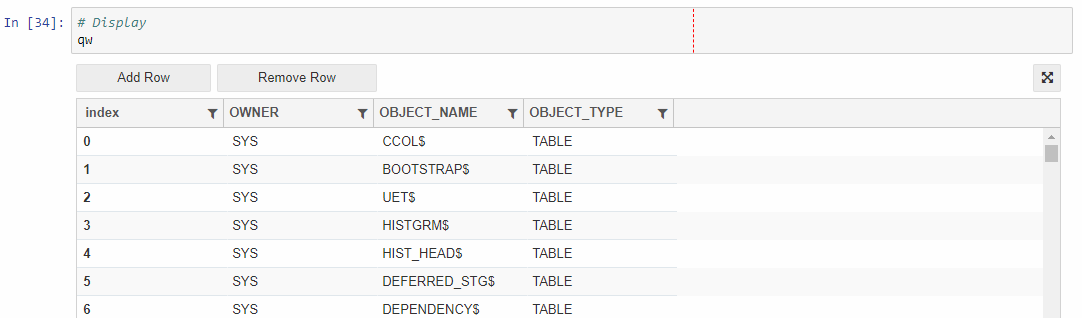
\includegraphics{img/CaptureQgrid.PNG}

Clicking on the header cells will sort the table by either ascending or
descending order. One can also filter the dataframe by clicking on the
"filter" icon: in this way you could inspect quickly all the ALMA
tables:

\begin{figure}
\centering
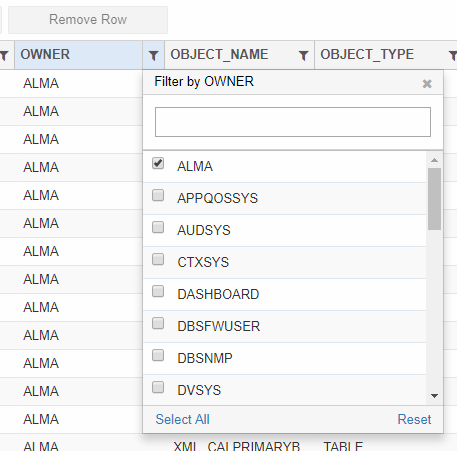
\includegraphics{img/CaptureQgrid2.PNG}
\caption{img}
\end{figure}

    \begin{Verbatim}[commandchars=\\\{\}]
{\color{incolor}In [{\color{incolor}17}]:} \PY{n}{sql\PYZus{}inspect\PYZus{}alma\PYZus{}tables} \PY{o}{=} \PY{l+s+s2}{\PYZdq{}\PYZdq{}\PYZdq{}}
         \PY{l+s+s2}{SELECT TABLE\PYZus{}NAME, COLUMN\PYZus{}NAME, COLUMN\PYZus{}ID, DATA\PYZus{}TYPE, DATA\PYZus{}LENGTH}
         \PY{l+s+s2}{    FROM DBA\PYZus{}TAB\PYZus{}COLUMNS}
         \PY{l+s+s2}{    WHERE OWNER = }\PY{l+s+s2}{\PYZsq{}}\PY{l+s+s2}{ALMA}\PY{l+s+s2}{\PYZsq{}}
         \PY{l+s+s2}{    ORDER BY TABLE\PYZus{}NAME}
         \PY{l+s+s2}{\PYZdq{}\PYZdq{}\PYZdq{}}
\end{Verbatim}


    \begin{Verbatim}[commandchars=\\\{\}]
{\color{incolor}In [{\color{incolor}18}]:} \PY{n}{cur}\PY{o}{.}\PY{n}{execute}\PY{p}{(}\PY{n}{sql\PYZus{}inspect\PYZus{}alma\PYZus{}tables}\PY{p}{)}
         \PY{n}{alma\PYZus{}tables\PYZus{}info} \PY{o}{=} \PY{n}{pd}\PY{o}{.}\PY{n}{DataFrame}\PY{p}{(}
             \PY{n}{cur}\PY{o}{.}\PY{n}{fetchall}\PY{p}{(}\PY{p}{)}\PY{p}{,} \PY{n}{columns}\PY{o}{=}\PY{p}{[}\PY{n}{rec}\PY{p}{[}\PY{l+m+mi}{0}\PY{p}{]} \PY{k}{for} \PY{n}{rec} \PY{o+ow}{in} \PY{n}{cur}\PY{o}{.}\PY{n}{description}\PY{p}{]}\PY{p}{)}
\end{Verbatim}


    \begin{Verbatim}[commandchars=\\\{\}]
{\color{incolor}In [{\color{incolor}19}]:} \PY{n}{qw\PYZus{}tables} \PY{o}{=} \PY{n}{qgrid}\PY{o}{.}\PY{n}{show\PYZus{}grid}\PY{p}{(}
             \PY{n}{alma\PYZus{}tables\PYZus{}info}\PY{o}{.}\PY{n}{sort\PYZus{}values}\PY{p}{(}\PY{n}{by}\PY{o}{=}\PY{p}{[}\PY{l+s+s1}{\PYZsq{}}\PY{l+s+s1}{TABLE\PYZus{}NAME}\PY{l+s+s1}{\PYZsq{}}\PY{p}{,} \PY{l+s+s1}{\PYZsq{}}\PY{l+s+s1}{COLUMN\PYZus{}ID}\PY{l+s+s1}{\PYZsq{}}\PY{p}{]}\PY{p}{)}\PY{p}{)}
         \PY{n}{qw\PYZus{}tables}
\end{Verbatim}


    
    \begin{verbatim}
QgridWidget(grid_options={'fullWidthRows': True, 'syncColumnCellResize': True, 'forceFitColumns': False, 'defa…
    \end{verbatim}

    
    \begin{Verbatim}[commandchars=\\\{\}]
{\color{incolor}In [{\color{incolor}20}]:} \PY{c+c1}{\PYZsh{} Let\PYZsq{}s get the last 5000 entries of the shiftlog}
         \PY{n}{sql} \PY{o}{=} \PY{l+s+s2}{\PYZdq{}\PYZdq{}\PYZdq{}}
         \PY{l+s+s2}{SELECT *}
         \PY{l+s+s2}{  FROM (SELECT *}
         \PY{l+s+s2}{        FROM ALMA.SHIFTLOG\PYZus{}ENTRIES}
         \PY{l+s+s2}{        ORDER BY SE\PYZus{}ID DESC)}
         \PY{l+s+s2}{ WHERE ROWNUM \PYZlt{}= 5000}
         \PY{l+s+s2}{\PYZdq{}\PYZdq{}\PYZdq{}}
\end{Verbatim}


    \begin{Verbatim}[commandchars=\\\{\}]
{\color{incolor}In [{\color{incolor} }]:} \PY{n}{cur}\PY{o}{.}\PY{n}{execute}\PY{p}{(}\PY{n}{sql}\PY{p}{)}
        \PY{k+kn}{import} \PY{n+nn}{pandas} \PY{k}{as} \PY{n+nn}{pd}
        
        \PY{n}{shift\PYZus{}log} \PY{o}{=} \PY{n}{pd}\PY{o}{.}\PY{n}{DataFrame}\PY{p}{(}
            \PY{n}{cur}\PY{o}{.}\PY{n}{fetchall}\PY{p}{(}\PY{p}{)}\PY{p}{,} \PY{n}{columns}\PY{o}{=}\PY{p}{[}\PY{n}{rec}\PY{p}{[}\PY{l+m+mi}{0}\PY{p}{]} \PY{k}{for} \PY{n}{rec} \PY{o+ow}{in} \PY{n}{cur}\PY{o}{.}\PY{n}{description}\PY{p}{]}\PY{p}{)}
\end{Verbatim}


    \begin{Verbatim}[commandchars=\\\{\}]
{\color{incolor}In [{\color{incolor} }]:} \PY{n}{shift\PYZus{}log}\PY{p}{[}\PY{n}{shift\PYZus{}log}\PY{o}{.}\PY{n}{SE\PYZus{}SUBJECT}\PY{o}{.}\PY{n}{str}\PY{o}{.}\PY{n}{contains}\PY{p}{(}\PY{l+s+s1}{\PYZsq{}}\PY{l+s+s1}{Full}\PY{l+s+s1}{\PYZsq{}}\PY{p}{)} \PY{o}{==} \PY{k+kc}{True}\PY{p}{]}
\end{Verbatim}


    \begin{Verbatim}[commandchars=\\\{\}]
{\color{incolor}In [{\color{incolor} }]:} \PY{n}{cur}\PY{o}{.}\PY{n}{execute}\PY{p}{(}\PY{n}{sql2}\PY{p}{)}
\end{Verbatim}


    \begin{Verbatim}[commandchars=\\\{\}]
{\color{incolor}In [{\color{incolor} }]:} \PY{n}{cur}\PY{o}{.}\PY{n}{execute}\PY{p}{(}\PY{l+s+s1}{\PYZsq{}}\PY{l+s+s1}{SELECT VIEW\PYZus{}NAME, OWNER from SYS.ALL\PYZus{}VIEWS order by OWNER, VIEW\PYZus{}NAME }\PY{l+s+s1}{\PYZsq{}}\PY{p}{)}
        \PY{n}{all\PYZus{}views\PYZus{}df} \PY{o}{=} \PY{n}{pd}\PY{o}{.}\PY{n}{DataFrame}\PY{p}{(}\PY{n}{cur}\PY{o}{.}\PY{n}{fetchall}\PY{p}{(}\PY{p}{)}\PY{p}{,} \PY{n}{columns}\PY{o}{=}\PY{p}{[}\PY{n}{rec}\PY{p}{[}\PY{l+m+mi}{0}\PY{p}{]} \PY{k}{for} \PY{n}{rec} \PY{o+ow}{in} \PY{n}{cur}\PY{o}{.}\PY{n}{description}\PY{p}{]}\PY{p}{)}
\end{Verbatim}


    \begin{Verbatim}[commandchars=\\\{\}]
{\color{incolor}In [{\color{incolor} }]:} \PY{n}{alltables} \PY{o}{=} \PY{n}{pd}\PY{o}{.}\PY{n}{DataFrame}\PY{p}{(}\PY{n}{cur}\PY{o}{.}\PY{n}{fetchall}\PY{p}{(}\PY{p}{)}\PY{p}{,} \PY{n}{columns}\PY{o}{=}\PY{p}{[}\PY{n}{rec}\PY{p}{[}\PY{l+m+mi}{0}\PY{p}{]} \PY{k}{for} \PY{n}{rec} \PY{o+ow}{in} \PY{n}{cur}\PY{o}{.}\PY{n}{description}\PY{p}{]}\PY{p}{)}
\end{Verbatim}


    \begin{Verbatim}[commandchars=\\\{\}]
{\color{incolor}In [{\color{incolor} }]:} \PY{n}{alltables}\PY{o}{.}\PY{n}{OWNER}\PY{o}{.}\PY{n}{unique}\PY{p}{(}\PY{p}{)}
\end{Verbatim}


    \begin{Verbatim}[commandchars=\\\{\}]
{\color{incolor}In [{\color{incolor} }]:} \PY{n}{alltables}\PY{o}{.}\PY{n}{query}\PY{p}{(}\PY{l+s+s1}{\PYZsq{}}\PY{l+s+s1}{OWNER == }\PY{l+s+s1}{\PYZdq{}}\PY{l+s+s1}{SPT}\PY{l+s+s1}{\PYZdq{}}\PY{l+s+s1}{\PYZsq{}}\PY{p}{)}
\end{Verbatim}


    \begin{Verbatim}[commandchars=\\\{\}]
{\color{incolor}In [{\color{incolor} }]:} \PY{n}{cur}\PY{o}{.}\PY{n}{execute}\PY{p}{(}\PY{l+s+s1}{\PYZsq{}}\PY{l+s+s1}{SELECT * FROM SOURCECATALOGUE.MEASUREMENTS}\PY{l+s+s1}{\PYZsq{}}\PY{p}{)}
\end{Verbatim}


    \begin{Verbatim}[commandchars=\\\{\}]
{\color{incolor}In [{\color{incolor} }]:} \PY{n}{measurements} \PY{o}{=} \PY{n}{pd}\PY{o}{.}\PY{n}{DataFrame}\PY{p}{(}\PY{n}{cur}\PY{o}{.}\PY{n}{fetchall}\PY{p}{(}\PY{p}{)}\PY{p}{,} \PY{n}{columns}\PY{o}{=}\PY{p}{[}\PY{n}{rec}\PY{p}{[}\PY{l+m+mi}{0}\PY{p}{]} \PY{k}{for} \PY{n}{rec} \PY{o+ow}{in} \PY{n}{cur}\PY{o}{.}\PY{n}{description}\PY{p}{]}\PY{p}{)}
\end{Verbatim}


    \begin{Verbatim}[commandchars=\\\{\}]
{\color{incolor}In [{\color{incolor} }]:} \PY{n}{cur}\PY{o}{.}\PY{n}{execute}\PY{p}{(}\PY{l+s+s1}{\PYZsq{}}\PY{l+s+s1}{SELECT * FROM SOURCECATALOGUE.MEASUREMENTS\PYZus{}LOG}\PY{l+s+s1}{\PYZsq{}}\PY{p}{)}
        \PY{n}{measurements\PYZus{}log} \PY{o}{=} \PY{n}{pd}\PY{o}{.}\PY{n}{DataFrame}\PY{p}{(}\PY{n}{cur}\PY{o}{.}\PY{n}{fetchall}\PY{p}{(}\PY{p}{)}\PY{p}{,} \PY{n}{columns}\PY{o}{=}\PY{p}{[}\PY{n}{rec}\PY{p}{[}\PY{l+m+mi}{0}\PY{p}{]} \PY{k}{for} \PY{n}{rec} \PY{o+ow}{in} \PY{n}{cur}\PY{o}{.}\PY{n}{description}\PY{p}{]}\PY{p}{)}
        \PY{n}{measurements\PYZus{}log}\PY{o}{.}\PY{n}{info}\PY{p}{(}\PY{p}{)}
\end{Verbatim}


    \begin{Verbatim}[commandchars=\\\{\}]
{\color{incolor}In [{\color{incolor} }]:} \PY{n}{measurements}\PY{o}{.}\PY{n}{info}\PY{p}{(}\PY{p}{)}
\end{Verbatim}


    \begin{Verbatim}[commandchars=\\\{\}]
{\color{incolor}In [{\color{incolor} }]:} \PY{n}{measurements}\PY{o}{.}\PY{n}{sort\PYZus{}values}\PY{p}{(}\PY{n}{by}\PY{o}{=}\PY{l+s+s1}{\PYZsq{}}\PY{l+s+s1}{UPDATE\PYZus{}DATE}\PY{l+s+s1}{\PYZsq{}}\PY{p}{,} \PY{n}{ascending}\PY{o}{=}\PY{k+kc}{False}\PY{p}{)}\PY{p}{[}\PY{p}{[}\PY{l+s+s1}{\PYZsq{}}\PY{l+s+s1}{MEASUREMENT\PYZus{}ID}\PY{l+s+s1}{\PYZsq{}}\PY{p}{,} \PY{l+s+s1}{\PYZsq{}}\PY{l+s+s1}{CATALOGUE\PYZus{}ID}\PY{l+s+s1}{\PYZsq{}}\PY{p}{,} \PY{l+s+s1}{\PYZsq{}}\PY{l+s+s1}{RA}\PY{l+s+s1}{\PYZsq{}}\PY{p}{,} \PY{l+s+s1}{\PYZsq{}}\PY{l+s+s1}{DEC}\PY{l+s+s1}{\PYZsq{}}\PY{p}{,} \PY{l+s+s1}{\PYZsq{}}\PY{l+s+s1}{FREQUENCY}\PY{l+s+s1}{\PYZsq{}}\PY{p}{,} \PY{l+s+s1}{\PYZsq{}}\PY{l+s+s1}{FLUX}\PY{l+s+s1}{\PYZsq{}}\PY{p}{,} \PY{l+s+s1}{\PYZsq{}}\PY{l+s+s1}{UPDATE\PYZus{}DATE}\PY{l+s+s1}{\PYZsq{}}\PY{p}{,} \PY{l+s+s1}{\PYZsq{}}\PY{l+s+s1}{DATE\PYZus{}OBSERVED}\PY{l+s+s1}{\PYZsq{}}\PY{p}{,} \PY{l+s+s1}{\PYZsq{}}\PY{l+s+s1}{ORIGIN}\PY{l+s+s1}{\PYZsq{}}\PY{p}{,} \PY{l+s+s1}{\PYZsq{}}\PY{l+s+s1}{EXECBLOCK\PYZus{}UID}\PY{l+s+s1}{\PYZsq{}}\PY{p}{]}\PY{p}{]}
\end{Verbatim}


    \begin{Verbatim}[commandchars=\\\{\}]
{\color{incolor}In [{\color{incolor} }]:} \PY{n}{cur}\PY{o}{.}\PY{n}{execute}\PY{p}{(}\PY{l+s+s1}{\PYZsq{}}\PY{l+s+s1}{select USERNAME from SYS.ALL\PYZus{}USERS order by USERNAME }\PY{l+s+s1}{\PYZsq{}}\PY{p}{)}
        \PY{n}{cur}\PY{o}{.}\PY{n}{fetchall}\PY{p}{(}\PY{p}{)}
\end{Verbatim}


    \begin{Verbatim}[commandchars=\\\{\}]
{\color{incolor}In [{\color{incolor} }]:} \PY{n}{cur}\PY{o}{.}\PY{n}{execute}\PY{p}{(}\PY{l+s+s1}{\PYZsq{}}\PY{l+s+s1}{select VIEW\PYZus{}NAME, OWNER from SYS.ALL\PYZus{}VIEWS order by OWNER, VIEW\PYZus{}NAME }\PY{l+s+s1}{\PYZsq{}}\PY{p}{)}
        \PY{n}{allviews} \PY{o}{=} \PY{n}{pd}\PY{o}{.}\PY{n}{DataFrame}\PY{p}{(}\PY{n}{cur}\PY{o}{.}\PY{n}{fetchall}\PY{p}{(}\PY{p}{)}\PY{p}{,} \PY{n}{columns}\PY{o}{=}\PY{p}{[}\PY{n}{rec}\PY{p}{[}\PY{l+m+mi}{0}\PY{p}{]} \PY{k}{for} \PY{n}{rec} \PY{o+ow}{in} \PY{n}{cur}\PY{o}{.}\PY{n}{description}\PY{p}{]}\PY{p}{)}
\end{Verbatim}


    \begin{Verbatim}[commandchars=\\\{\}]
{\color{incolor}In [{\color{incolor} }]:} \PY{n}{allviews}
\end{Verbatim}


    \begin{Verbatim}[commandchars=\\\{\}]
{\color{incolor}In [{\color{incolor} }]:} \PY{n}{cur}\PY{o}{.}\PY{n}{execute}\PY{p}{(}\PY{l+s+s2}{\PYZdq{}}\PY{l+s+s2}{SELECT * FROM ALL\PYZus{}TAB\PYZus{}COLUMNS where table\PYZus{}name = }\PY{l+s+s2}{\PYZsq{}}\PY{l+s+s2}{SHIFTLOG\PYZus{}ENTRIES}\PY{l+s+s2}{\PYZsq{}}\PY{l+s+s2}{\PYZdq{}}\PY{p}{)}
\end{Verbatim}


    \begin{Verbatim}[commandchars=\\\{\}]
{\color{incolor}In [{\color{incolor} }]:} \PY{n}{table\PYZus{}info} \PY{o}{=} \PY{n}{pd}\PY{o}{.}\PY{n}{DataFrame}\PY{p}{(}\PY{n}{cur}\PY{o}{.}\PY{n}{fetchall}\PY{p}{(}\PY{p}{)}\PY{p}{,} \PY{n}{columns}\PY{o}{=}\PY{p}{[}\PY{n}{rec}\PY{p}{[}\PY{l+m+mi}{0}\PY{p}{]} \PY{k}{for} \PY{n}{rec} \PY{o+ow}{in} \PY{n}{cur}\PY{o}{.}\PY{n}{description}\PY{p}{]}\PY{p}{)}
\end{Verbatim}


    \begin{Verbatim}[commandchars=\\\{\}]
{\color{incolor}In [{\color{incolor} }]:} \PY{n}{table\PYZus{}info}
\end{Verbatim}


    \begin{Verbatim}[commandchars=\\\{\}]
{\color{incolor}In [{\color{incolor} }]:} \PY{n}{shift\PYZus{}log}\PY{o}{.}\PY{n}{head}\PY{p}{(}\PY{p}{)}
\end{Verbatim}


    \begin{Verbatim}[commandchars=\\\{\}]
{\color{incolor}In [{\color{incolor} }]:} \PY{n}{shift\PYZus{}log}\PY{o}{.}\PY{n}{info}\PY{p}{(}\PY{p}{)}
\end{Verbatim}


    \begin{Verbatim}[commandchars=\\\{\}]
{\color{incolor}In [{\color{incolor} }]:} \PY{n}{shift\PYZus{}log}\PY{o}{.}\PY{n}{query}\PY{p}{(}\PY{l+s+s1}{\PYZsq{}}\PY{l+s+s1}{SE\PYZus{}TYPE == 1}\PY{l+s+s1}{\PYZsq{}}\PY{p}{)}\PY{p}{[}\PY{p}{[}\PY{l+s+s1}{\PYZsq{}}\PY{l+s+s1}{SE\PYZus{}TIMESTAMP}\PY{l+s+s1}{\PYZsq{}}\PY{p}{,} \PY{l+s+s1}{\PYZsq{}}\PY{l+s+s1}{SE\PYZus{}SHIFTACTIVITY}\PY{l+s+s1}{\PYZsq{}}\PY{p}{,} \PY{l+s+s1}{\PYZsq{}}\PY{l+s+s1}{SE\PYZus{}LOCATION}\PY{l+s+s1}{\PYZsq{}}\PY{p}{]}\PY{p}{]}
\end{Verbatim}


    \begin{Verbatim}[commandchars=\\\{\}]
{\color{incolor}In [{\color{incolor} }]:} \PY{n}{shift\PYZus{}log}\PY{o}{.}\PY{n}{query}\PY{p}{(}\PY{l+s+s1}{\PYZsq{}}\PY{l+s+s1}{SE\PYZus{}TYPE == 2}\PY{l+s+s1}{\PYZsq{}}\PY{p}{)}
\end{Verbatim}


    \begin{Verbatim}[commandchars=\\\{\}]
{\color{incolor}In [{\color{incolor}21}]:} \PY{n}{cur}\PY{o}{.}\PY{n}{close}\PY{p}{(}\PY{p}{)}
         \PY{n}{con}\PY{o}{.}\PY{n}{close}\PY{p}{(}\PY{p}{)}
\end{Verbatim}



    % Add a bibliography block to the postdoc
    
    
    
    \end{document}
